\documentclass[journal]{IEEEtran}
\IEEEoverridecommandlockouts
\usepackage{etoolbox}
\makeatletter
\patchcmd{\abstract}{---}{-}{}{}
\patchcmd{\IEEEkeywords}{---}{-}{}{}
\makeatother
\usepackage{cite}
\usepackage{amsmath,amssymb,amsfonts}
\usepackage{algorithmic}
\usepackage{graphicx}
\usepackage{textcomp}
\usepackage{xcolor}
\usepackage{colortbl}
\usepackage{booktabs}
\usepackage{multirow}
\usepackage{balance}
\usepackage[hidelinks]{hyperref}
\usepackage{microtype}
\usepackage{tikz}
\usetikzlibrary{arrows, positioning, calc}

\def\BibTeX{{\rm B\kern-.05em{\sc i\kern-.025em b}\kern-.08em
    T\kern-.1667em\lower.7ex\hbox{E}\kern-.125emX}}

\begin{document}

\title{Multilingual Spam Email Detection for English and Bangla Messages using QLoRA-Fine-Tuned Large Language Models with Explainable AI Validation}

\author{Najmush Shakib and Munim Halder \\
\textit{Department of Computer Science and Engineering} \\
\textit{Bangladesh University of Business and Technology (BUBT)} \\
Dhaka, Bangladesh \\
nstasin81@gmail.com, munimhalder666@gmail.com
}

\maketitle

\begin{abstract}
Global messaging platforms are experiencing a surge in spam, phishing, and smishing attacks, which impose significant financial and security costs on users. While current spam detection algorithms perform exceptionally well for resource-rich languages like English, low-resource languages such as Bangla (with over 230 million speakers) lack robust support from commercial and academic filters. To bridge this gap, this paper introduces a unified multilingual framework that classifies both English and Bangla spam simultaneously. This approach eliminates the need for language-specific feature engineering or separate processing pipelines. We utilized Quantized Low-Rank Adaptation (QLoRA) to fine-tune five compact, pre-trained Large Language Models (ranging from Phi-3.5 Mini to SmolLM2-360M) on a combined dataset of standard SMS spam and native Bangla phishing messages. Our preprocessing pipeline incorporates Unicode normalization, URL token substitution, and a group-aware splitting strategy designed to prevent data leakage during training. We applied the Synthetic Minority Over-sampling Technique (SMOTE) exclusively within the training feature space to balance classes without compromising the validation sets. Model performance was evaluated using standard metrics across both languages, and McNemar's test was used to verify the statistical significance of the results. Additionally, an Explainable AI (XAI) module based on cross-layer attention aggregation was included to ensure that predictions rely on semantically relevant features rather than superficial artifacts. The experimental results show that fine-tuning compact LLMs via QLoRA is a highly parameter-efficient approach, achieving a peak accuracy of 98.24\% on the bilingual task and outperforming traditional machine learning baselines.
\end{abstract}

\begin{IEEEkeywords}
Spam Detection, Bangla NLP, QLoRA, Large Language Models, Parameter-Efficient Fine-Tuning, PEFT, Explainable AI, Multilingual Classification, Phishing Detection, Smishing
\end{IEEEkeywords}

\section{Introduction}

\subsection{Background and Motivation}

\IEEEPARstart{U}{nwanted} electronic messages, or spam, are a massive security and economic headache in today's digital world. It's not just annoying to get spam; it's actually the main way that attackers launch phishing scams, spread malware, and commit financial fraud. This costs billions of dollars every year~\cite{ref1}. The problem has only gotten worse with the explosion of mobile messaging apps like WhatsApp and SMS. Scammers are also getting smarter. They mix up their language, use slang, and switch between different languages in the same message, which completely breaks older keyword-based spam filters~\cite{ref5},~\cite{ref6}.

Lately, there have been some great strides in natural language processing (NLP) and machine learning. We now have really strong spam classifiers that use everything from basic statistical features to advanced transformer models~\cite{ref4},~\cite{ref7},~\cite{ref9}. Because of this, English spam detection is basically a solved problem in academia, with many systems hitting over 98\% accuracy on standard datasets like the SMS Spam Collection~\cite{ref1} and Enron Email~\cite{ref9}. But there is a catch: these models usually only work well on one language at a time.

This is a huge problem for languages like Bangla. Even though millions of people speak it, it doesn't get nearly as much attention in the AI community. To make things harder, people in Bangladesh rarely type in pure Bangla. They mix native script with English words, use Romanized spellings, and switch languages mid-sentence. At the same time, mobile money services like bKash and Nagad have become incredibly popular, leading to a wave of highly localized phishing attacks. Standard Bangla text classifiers might look good on paper~\cite{ref7}, but they often fail when faced with these messy, real-world threats.

\subsection{Problem Statement}

Right now, research seems split into two camps. On one side, you have highly advanced English models. On the other side, you have separate, smaller models built just for local dialects. A lot of the systems designed for Bangla need huge amounts of labeled data or custom feature extractors that break as soon as scammers change their tactics~\cite{ref7},~\cite{ref10}. As far as we know, there isn't a single system out there that can handle both English and Bangla spam simultaneously without needing completely separate processing steps for each language.

Having separate models for different languages is a nightmare for real-world companies. If a telecom provider or a bank wants to filter spam, running a separate pipeline for English and another for Bangla adds a lot of unnecessary cost, lag, and maintenance headaches. What the industry actually needs is a single, unified model that can read raw text in multiple languages and explain why it flagged a message.

\subsection{Proposed Solution and Contributions}

In this paper, we try to solve this by building a single framework that detects spam across both languages. We took some publicly available, smaller Large Language Models (LLMs) and fine-tuned them using Quantized Low-Rank Adaptation (QLoRA)~\cite{ref11}. The great thing about QLoRA is that it lets you train massive models by only tweaking a tiny fraction of their weights. This cuts down the memory needed so much that we could run the training on a normal consumer GPU. This kind of cost-saving approach is a game-changer for low-resource languages, where building a model from scratch is usually too expensive.

The primary contributions of this paper are:

\textbf{1) Unified Bilingual Framework:} We built a single pipeline using an LLM that catches spam in both English and Bangla, without needing separate rules or extractors for each language.

\textbf{2) Leakage-Free Dataset Splits:} We sorted our Bangla data based on message templates before splitting it into training and testing sets. This makes sure the model doesn't just memorize similar messages, fixing a major data leakage issue that a lot of previous studies missed.

\textbf{3) Fair Multi-Model Comparison:} We took five different LLMs (ranging from 360 million to 3.8 billion parameters) and fine-tuned all of them under the exact same conditions to see which size and architecture actually works best.

\textbf{4) Seeing Inside the Model:} We added a way to track the model's attention weights across its layers. This lets us pull out importance scores for specific words, proving that the model is actually reading the text and not just guessing based on random artifacts.

\textbf{5) Statistical Checks:} We ran McNemar's test on our results to make sure that the performance differences between the models are statistically real, and not just lucky random flukes.



\section{Related Work}

People have been trying to classify spam and phishing messages for a long time. Early work using the SMS Spam Collection dataset mostly relied on older algorithms like Support Vector Machines (SVM) and Naïve Bayes~\cite{ref1},~\cite{ref5}. They got pretty high accuracy numbers, but they didn't really "understand" the text. Later, researchers tried building custom feature sets just for catching phishing URLs~\cite{ref2},~\cite{ref8}. While these worked well in a lab, scammers quickly learned to bypass them by hiding their code or using non-HTML tricks.

Eventually, the focus shifted to neural networks. For example, Dutta~\cite{ref3} used RNN-LSTMs to catch brand-new phishing URLs, and the team behind SpamDL~\cite{ref9} mixed GloVe word embeddings with Bi-LSTMs to sort emails. In the mobile world, mixed systems like SmishGuard~\cite{ref6} pushed detection rates even higher. The downside to all of these? They were built strictly for English. If you threw another language at them, they wouldn't know what to do.

When it comes to Bangla text, researchers have started looking at multilingual transformer models. Alam et al.~\cite{ref4} tested out mBERT and XLM-RoBERTa, but they noticed that breaking words down into smaller subwords often ruins the meaning for languages with less data. Talukder et al.~\cite{ref7} actually got fantastic results on Bangla SMS messages using a mix of BiLSTM and 1D-CNNs. But again, their setup was entirely restricted to Bangla.

\subsection{Synthesis and Research Gap}

Looking at past research, there's an obvious divide. English spam detection gets all the advanced, highly accurate models, while research on Bangla is stuck playing catch-up with smaller datasets and older architectures. As far as we can tell, no one has actually managed to train one single model to effectively handle both languages at the same time.

We also noticed a few repeating issues in past studies. Many researchers didn't account for data leakage when dealing with template-based messages. They also stuck purely to monolingual datasets, and almost none of them built in any way to explain the model's decisions, which is a big deal if you actually want to use the system in real-world cybersecurity. Table~\ref{tab:comparative} lays out a quick comparison of these past works.

\begin{table}[htbp]
\caption{Comparative Summary of Methods}
\label{tab:comparative}
\centering
\begin{tabular}{lllc}
\toprule
\textbf{Ref.} & \textbf{Dataset} & \textbf{Architecture} & \textbf{Acc.} \\
\midrule
\cite{ref1} & SMS Spam Collection (5,574) & SVM, NB & 97.64\% \\
\cite{ref2} & 6,000 URLs & XGBoost & 99.17\% \\
\cite{ref3} & PhishTank ($\sim$13k URLs) & RNN-LSTM & 97.40\% \\
\cite{ref4} & 6 Bangla datasets & mBERT & 93.80\% \\
\cite{ref5} & SMS Spam v1 (5,169) & NB + Dict. & 96.20\% \\
\cite{ref6} & SMS Phishing (7,261) & XGBoost & 98.47\% \\
\cite{ref7} & 11,599 Bangla SMS & BiLSTM & 99.00\% \\
\cite{ref8} & URL phishing DB & SVM, LR & 91.40\% \\
\cite{ref9} & Enron + SpamAssassin & Bi-LSTM & $\sim$98\% \\
\cite{ref10} & 84,000 global SMS & Multi-NLP & 97.89\% \\
\textbf{Ours} & \textbf{Eng + Bangla (7,924)} & \textbf{QLoRA LLM} & \textbf{98.24\%} \\
\bottomrule
\end{tabular}
\end{table}

We wanted to fix these problems. So, we put together a bilingual dataset, created a way to split the data without leaking templates, used efficient fine-tuning to tap into the power of pretrained LLMs, and finally, added explainable AI features so we could see what the model is thinking.



\section{Methodology}

This section details the experimental setup and formalizes the learning task. The methodology consists of five main phases: (A) problem formulation, (B) dataset preparation, (C) preprocessing, (D) data splitting and leakage prevention, and (E) architecture design and training.

\subsection{Problem Formulation}

The task of multilingual spam detection is modeled as a supervised binary sequence classification problem. Let $\mathcal{D} = \{(x_i, y_i)\}_{i=1}^{N}$ denote a dataset consisting of $N$ text messages, where each message $x_i$ is a sequence of tokens from a vocabulary $\mathcal{V}$ that spans multiple languages (in this context, English and Bangla). The corresponding label $y_i \in \{0, 1\}$ denotes whether the message is legitimate (ham, $y_i = 0$) or malicious (spam/phishing, $y_i = 1$). 

The objective is to learn a mapping function $f_\theta: \mathcal{X} \rightarrow \mathcal{Y}$, parameterized by $\theta$, such that the predicted label $\hat{y}_i = f_\theta(x_i)$ minimizes the standard cross-entropy loss over the dataset:
\begin{equation}
\mathcal{L}(\theta) = -\frac{1}{N} \sum_{i=1}^{N} \left[ y_i \log f_\theta(x_i) + (1 - y_i) \log (1 - f_\theta(x_i)) \right]
\end{equation}
Unlike traditional approaches that require language-identification branching, $f_\theta$ must inherently capture cross-lingual semantic representations within a unified embedding space. In this work, $f_\theta$ represents a pre-trained causal language model adapted for classification, and we seek to find optimal parameters $\theta^*$ using a low-rank approximation strategy to minimize computational overhead.

\begin{figure}[htbp]
\centering
\resizebox{\columnwidth}{!}{
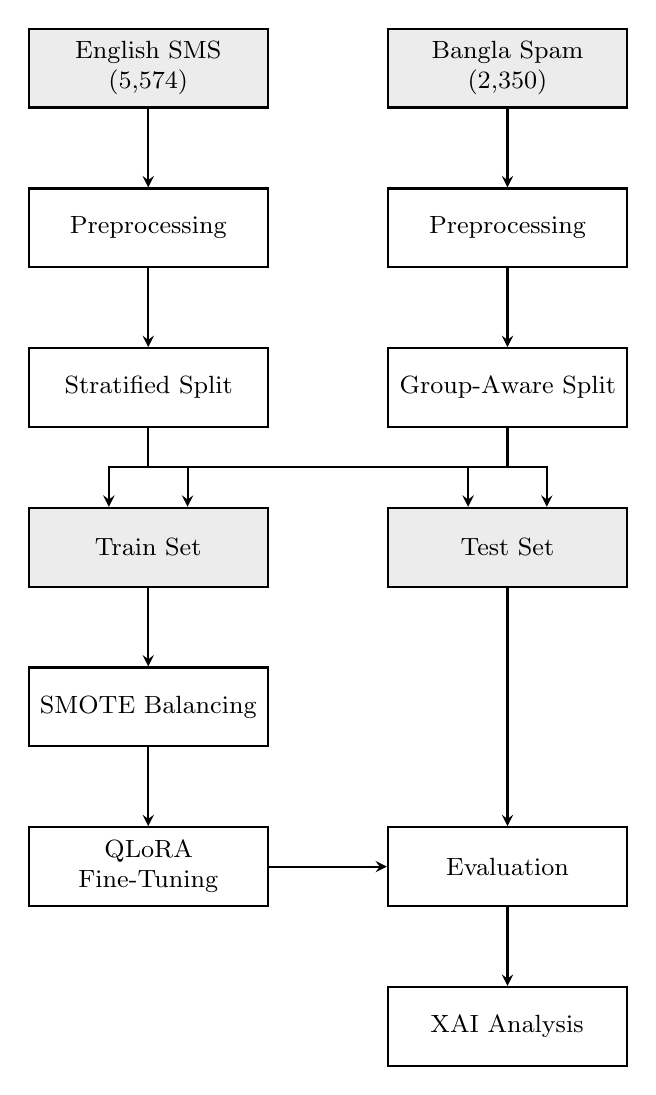
\begin{tikzpicture}[
    node distance=1cm and 1.5cm,
    box/.style={rectangle, draw=black, thick, fill=white, minimum width=3cm, minimum height=1cm, text centered, text width=2.8cm, font=\small},
    data/.style={rectangle, draw=black, thick, fill=gray!15, minimum width=3cm, minimum height=1cm, text centered, text width=2.8cm, font=\small},
    arrow/.style={thick, ->, >=stealth, draw=black}
]
\node (eng) [data] {English SMS\\(5,574)};
\node (ben) [data, right=1.5cm of eng] {Bangla Spam\\(2,350)};
\node (prep_eng) [box, below=of eng] {Preprocessing};
\node (prep_ben) [box, below=of ben] {Preprocessing};
\node (split_eng) [box, below=of prep_eng] {Stratified Split};
\node (split_ben) [box, below=of prep_ben] {Group-Aware Split};
\node (train) [data, below=1cm of split_eng] {Train Set};
\node (test) [data, below=1cm of split_ben] {Test Set};
\node (smote) [box, below=of train] {SMOTE Balancing};
\node (qlora) [box, below=of smote] {QLoRA Fine-Tuning};
\node (eval) [box] at (test |- qlora) {Evaluation};
\node (xai) [box, below=of eval] {XAI Analysis};

\draw [arrow] (eng) -- (prep_eng);
\draw [arrow] (ben) -- (prep_ben);
\draw [arrow] (prep_eng) -- (split_eng);
\draw [arrow] (prep_ben) -- (split_ben);
\draw [arrow] (split_eng.south) -- ++(0,-0.5) -| ([xshift=-0.5cm]train.north);
\draw [arrow] (split_eng.south) -- ++(0,-0.5) -| ([xshift=-0.5cm]test.north);
\draw [arrow] (split_ben.south) -- ++(0,-0.5) -| ([xshift=0.5cm]train.north);
\draw [arrow] (split_ben.south) -- ++(0,-0.5) -| ([xshift=0.5cm]test.north);
\draw [arrow] (train) -- (smote);
\draw [arrow] (smote) -- (qlora);
\draw [arrow] (test) -- (eval);
\draw [arrow] (qlora) -- (eval);
\draw [arrow] (eval) -- (xai);
\end{tikzpicture}
}
\caption{End-to-End Methodology Framework}
\label{fig:methodology}
\end{figure}

\subsection{Dataset Construction and Description}

The study uses two distinct corpora that are combined into a single
bilingual training and evaluation dataset.

\textit{1) English Corpus - SMS Spam Collection:} The English portion of the dataset is derived from the SMS Spam Collection dataset introduced by Almeida et al.~\cite{ref1}. This data set contains 5,574 SMS messages in
English, which are hand-labeled to be either ``ham'' or ``spam.'' The dataset exhibits significant class imbalance: approximately 86.6\% of the messages are legitimate (ham), while 13.4\% are spam; this
distribution closely mirrors real-world communication flows, necessitating
effective class balancing techniques. The messages in this data set are stored as
plain UTF-8 strings.

\textit{2) Bangla Corpus - Phishing and Promotional Spam Dataset:} The
Bangla dataset comprises a native language corpus of phishing and
promotional spam gathered from Bangladesh digital communication
platforms. The dataset includes messages representing various
categories of malware, including MFS fraud, phishing messages under the
guise of bKash and Nagad, lottery, prize and promotional spam, as well
as transactional and conversational messages, which constitute the ham
category. Every message entry in the Bangla dataset includes a template\_id field indicating its foundational template. This attribute enables the group-aware
splitting technique discussed in Section III-C. The labeling scheme for
the binary classification task is identical to the one for the English
dataset -- 0 represents ham, while 1 indicates spam.

The summary of both datasets prior to preprocessing is shown in Table
II.

\begin{table}[htbp]
\caption{Dataset Composition Before Preprocessing}
\label{tab:dataset_raw}
\centering
\begin{tabular}{lll}
\toprule
\textbf{Attribute} & \textbf{English (SMS Spam)} & \textbf{Bangla (Phishing/Spam)} \\
\midrule
Total Records & 5,574 & 2,350 \\
Ham (Label = 0) & $\sim$4,827 & 810 \\
Spam (Label = 1) & $\sim$747 & 1,540 \\
Language & English & Bangla (code-mixed) \\
Source & Public repo \cite{ref1} & Native corpus \\
Template Metadata & None & template\_id per record \\
\bottomrule
\end{tabular}
\end{table}

\subsection{Preprocessing Pipeline}

The main goal of our preprocessing was just to keep the text formatting consistent between English and Bangla. We specifically avoided heavy editing like stemming or removing stop-words. In spam detection, those little words often carry important context, and stripping them out can totally mess up how multilingual tokenizers read Bangla script.

\textit{1) Cleaning up formatting:} We started by cleaning up the messy raw text. We swapped out newlines (\textbackslash n), carriage returns (\textbackslash r), and tabs (\textbackslash t) for basic spaces, and trimmed off any extra spaces at the beginning or end of the messages to get a clean baseline.

\textit{2) Normalizing Unicode:} Mixing different alphabets usually causes weird encoding glitches. To fix this, we ran all the text through NFKC normalization in Python. This basically breaks down weird characters into their standard forms and puts them back together, making sure everything is uniformly encoded before the tokenizer sees it.

\textit{3) Hiding URLs and Numbers:} Phishing campaigns love to hide behind unique, randomized URLs. Instead of letting the model get confused by thousands of unique web addresses, we used regular expressions to swap out any \texttt{http}, \texttt{https}, or \texttt{www} links with a simple \texttt{URL} tag. We did the same thing for random digits, swapping them with a \texttt{NUMBER} tag. This keeps the model aware that a link or number was there without flooding its vocabulary with random text.

\textit{4) Dropping Duplicates and Blanks:} We simply threw out any rows that were missing text or labels. If a message showed up multiple times as an exact duplicate, we kept the first one and deleted the rest. The number
of records before and after each cleaning step is shown in Table~\ref{tab:dataset_prep}
below.

\begin{table}[htbp]
\caption{Record Counts After Each Preprocessing Stage}
\label{tab:dataset_prep}
\centering
\begin{tabular}{lcc}
\toprule
\textbf{Stage} & \textbf{English Records} & \textbf{Bangla Records} \\
\midrule
Raw & 5,574 & 2,350 \\
After Null Removal & 5,500 & 2,280 \\
After Deduplication & 5,170 & 2,205 \\
Final & 5,170 & 2,205 \\
\bottomrule
\end{tabular}
\end{table}

\textit{5) Checking Labels:} Finally, we ran a quick script to make sure every single label was either a 0 (for ham) or a 1 (for spam). No unexpected values slipped through.

\subsection{Data Partitioning and Leakage Prevention}

We couldn't just do a standard random split on the data. The Bangla dataset has a lot of messages built from the exact same templates. If we randomly split the data, parts of the same template would end up in both the training and test sets. This creates data leakage, where the model just memorizes the template structure instead of actually learning how to spot a threat.

\textit{1) Splitting Bangla by Group:} To prevent this, we used scikit-learn's \texttt{GroupShuffleSplit} and told it to group everything by the \texttt{template\_id}. This way, every single variation of a specific template went entirely into the training set or entirely into the test set. We kept 20\% for testing, and checked afterward to confirm that absolutely no templates crossed over.

\textit{2) English: Stratified Random Splitting:} Since the English corpus
does not contain template metadata, stratified random splitting with 20\%
test size and the same seed was applied to the corpus. Stratification
according to the label column ensures that the spam-to-ham class distribution in the training subset mirrors the overall English corpus.

\textit{3) Combination and Shuffle:} The English and Bangla training data
splits were joined together and randomly shuffled (random\_state=42) to
create one bilingual training dataset. The same process was applied to
the test data splits. The shuffle operation ensures that no model can
exploit any positional information linked to the order in
which the language-specific data splits were created. The dataset was
finally converted into Hugging Face Datasets for use with the Trainer
API in the later stages.

\textit{4) Leakage Verification:} The following are the three tests done
independently to verify the absence of any kind of leakage during the
partitioning process:

(a) Exact match intersection of the train and test text strings.

(b) Template intersection of the set of Bangla training and test
templates.

(c) TF-IDF vectorization in the SMOTE phase trained only on the
training partition.

All three of these verification steps independently confirmed exactly zero data leakage between the final training and testing partitions, ensuring the integrity of the evaluation metrics.

\subsection{Class Imbalance Handling via SMOTE}

The merged training dataset retains the inherent class imbalance of the source corpora, with legitimate messages significantly outnumbering spam examples. Training a classification model directly on this imbalanced distribution induces a majority-class bias, yielding artificially high overall accuracy while severely degrading recall on the minority spam class---the critical metric for threat detection.

To mitigate this imbalance, the Synthetic Minority Over-sampling Technique (SMOTE) was applied exclusively to the training partition.
SMOTE synthesizes minority class instances through interpolation in the
feature space of real minority instances and their k nearest neighbors.
To prevent test-set contamination during LLM fine-tuning, SMOTE had to be run in the TF-IDF feature space using a vectorizer
trained on the training data set alone using a vocabulary of 5,000
features; the resampled indices were then used to adjust the
distribution of training data set. The test data set was vectorized
using the fitted but not the refitted vectorizer from the training data
set to reflect an actual inference scenario. Table~\ref{tab:smote} provides a summary
of the class distribution prior to and after running SMOTE.

\begin{table}[htbp]
\caption{Training Set Class Distribution Before and After SMOTE}
\label{tab:smote}
\centering
\begin{tabular}{lcc}
\toprule
\textbf{Class} & \textbf{Before SMOTE} & \textbf{After SMOTE} \\
\midrule
Ham (0) & 4,216 & 4,216 \\
Spam (1) & 1,684 & 4,216 \\
\textbf{Total} & \textbf{5,900} & \textbf{8,432} \\
\bottomrule
\end{tabular}
\end{table}

\subsection{Model Architectures and Selection Rationale}

Five distinct pre-trained Large Language Models (LLMs) were selected as base architectures. To ensure efficient token processing in Bangla, selection was restricted to models pre-trained on diverse multilingual corpora. Table~\ref{tab:models} outlines the selected models, all of which are publicly hosted on the Hugging Face Hub.

\begin{table}[htbp]
\caption{Selected Pretrained LLMs}
\label{tab:models}
\centering
\begin{tabular}{llc}
\toprule
\textbf{Model Name} & \textbf{Hugging Face ID} & \textbf{Parameters} \\
\midrule
Phi-3.5 Mini & microsoft/Phi-3.5-mini-instruct & $\sim$3.8B \\
Qwen2.5-1.5B & Qwen/Qwen2.5-1.5B-Instruct & $\sim$1.5B \\
TinyLlama-1.1B & TinyLlama/TinyLlama-1.1B-Chat-v1.0 & $\sim$1.1B \\
StableLM-2-1.6B & stabilityai/stablelm-2-1\_6b-chat & $\sim$1.6B \\
SmolLM2-360M & HuggingFaceTB/SmolLM2-360M-Instruct & $\sim$360M \\
\bottomrule
\end{tabular}
\end{table}

Model selection was guided by specific operational constraints. First, candidate architectures were restricted to parameter sizes viable for fine-tuning on a single consumer-grade GPU. Second, instruction-tuned variants were prioritized, as they generally provide superior zero-shot initialization for classification tasks compared to raw foundational models. Finally, the selection intentionally spans a broad parameter continuum---from 360 million to 3.8 billion---to empirically evaluate the scaling relationship between computational efficiency and classification accuracy.

\subsection{QLoRA Fine-Tuning Configuration}

Binary sequence classification fine-tuning was executed using Quantized Low-Rank Adaptation (QLoRA) \cite{ref11}. QLoRA integrates 4-bit weight quantization with low-rank adapters, facilitating the parameter-efficient adaptation of large-scale models within constrained memory footprints. The
particular quantization parameters used included Normal Float 4-bit
(nf4) quantization with double quantization set to True and fp16 for
activation tensors computations.

Adapter layers based on LoRA technology were embedded into the attention
projection matrices for each model. The target modules were selected
according to the naming convention of each model:
\begin{itemize}
    \item \textbf{Phi-3.5 Mini:} qkv\_proj, o\_proj, gate\_up\_proj, down\_proj
    \item \textbf{Qwen2.5 and StableLM-2:} q\_proj, k\_proj, v\_proj, o\_proj, gate\_proj, up\_proj, down\_proj
    \item \textbf{TinyLlama and SmolLM2:} q\_proj, k\_proj, v\_proj, o\_proj
\end{itemize}

The LoRA rank value was equal to r=16, the scale factor was set to
alpha=32, while the dropout probability was chosen to be equal to 0.05
resulting in less than 1\% of total model parameters being trainable.

\begin{table}[htbp]
\caption{QLoRA Hyperparameter Configuration}
\label{tab:qlora}
\centering
\begin{tabular}{ll}
\toprule
\textbf{Hyperparameter} & \textbf{Value} \\
\midrule
Quantization & 4-bit NF4 w/ double quant \\
Compute dtype & float16 \\
LoRA rank (r) & 16 \\
LoRA alpha & 32 \\
LoRA dropout & 0.05 \\
Target modules & Architecture-specific \\
Trainable params & $<$ 1\% of total \\
Task type & SEQ\_CLS \\
\bottomrule
\end{tabular}
\end{table}

\subsection{Training Protocol and Hyperparameters}

Models were trained via the Hugging Face Trainer API with an effective batch size of 8 (4 per device with 2 accumulation steps) for 1 epoch. We utilized the Paged AdamW 8-bit optimizer with a learning rate of $2 \times 10^{-4}$. Mixed precision (fp16) and gradient checkpointing were enabled to minimize memory footprint. Maximum sequence length was dynamically bounded between 128 and 256 tokens based on the 95th percentile of the training distribution. At the end of the epoch, models were evaluated on the tokenized test dataset, generating complete classification logits.



\section{Results and Discussion}

All five models were evaluated against the bilingual test partition. Predictions were derived using the argmax of the output logit vector. Evaluation metrics included overall accuracy, precision, recall, and F1 score, alongside language-stratified measurements to isolate performance variations across subsets.

\subsection{Aggregate Model Performance}

Table~\ref{tab:aggregate_results} presents the aggregate performance of all five models on the combined bilingual test set.

\begin{table}[htbp]
\caption{Aggregate Performance of Fine-Tuned Models on the Combined Bilingual Test Set}
\label{tab:aggregate_results}
\centering
\begin{tabular}{lcccc}
\toprule
\textbf{Model} & \textbf{Overall Acc.} & \textbf{Precision} & \textbf{Recall} & \textbf{F1 (Spam)} \\
\midrule
\rowcolor{gray!20} \textbf{Qwen2.5-1.5B} & \textbf{98.24\%} & \textbf{0.974} & \textbf{0.964} & \textbf{0.969} \\
Phi-3.5 Mini & 98.17\% & 0.974 & 0.962 & 0.968 \\
TinyLlama-1.1B & 97.76\% & 0.958 & 0.964 & 0.961 \\
StableLM-2-1.6B & 97.56\% & 0.953 & 0.962 & 0.957 \\
SmolLM2-360M & 96.20\% & 0.921 & 0.948 & 0.934 \\
\bottomrule
\end{tabular}
\end{table}



The empirical results demonstrate that all evaluated architectures achieved high bilingual classification accuracy after QLoRA adaptation, reinforcing the effectiveness of low-rank updates for complex cross-lingual tasks. Interestingly, overall accuracy does not strictly correlate with parameter volume. Factors such as the quality of multilingual pre-training data, attention mechanism architecture, and the tokenizer's coverage of the Bangla script appear to heavily influence final performance.

The peak accuracy of 98.24\% (F1: 0.969) closely matches state-of-the-art monolingual baselines like SmishGuard~\cite{ref6} (98.47\%), despite operating in a vastly more complex, unsegregated bilingual space.

\subsection{Language-Stratified Performance Analysis}

Table~\ref{tab:lang_results} disaggregates the performance of each model along the English
and Bangla dimensions of the test set, providing a more granular
characterization of bilingual generalization.

\begin{table}[htbp]
\caption{Per-Language Performance Breakdown}
\label{tab:lang_results}
\centering
\begin{tabular}{lcccc}
\toprule
\textbf{Model} & \textbf{English Acc.} & \textbf{English F1} & \textbf{Bangla Acc.} & \textbf{Bangla F1} \\
\midrule
\rowcolor{gray!20} \textbf{Qwen2.5-1.5B} & \textbf{99.03\%} & \textbf{0.961} & \textbf{96.37\%} & \textbf{0.972} \\
Phi-3.5 Mini & 99.32\% & 0.973 & 95.46\% & 0.965 \\
TinyLlama-1.1B & 98.74\% & 0.951 & 95.46\% & 0.966 \\
StableLM-2-1.6B & 99.03\% & 0.962 & 94.10\% & 0.955 \\
SmolLM2-360M & 98.26\% & 0.931 & 91.38\% & 0.936 \\
\bottomrule
\end{tabular}
\end{table}



Stratified analysis reveals minor performance degradation on the Bangla subset across all models. This is likely attributable to suboptimal coverage of the Bangla script by standard multilingual tokenizers. Nevertheless, the sustained high accuracy (e.g., Qwen2.5-1.5B achieving 96.37\% on Bangla) indicates that pretrained multilingual representations can successfully accommodate disparate scripts within a unified embedding space.

Performance variations between the English and Bangla subsets provide insights into tokenization efficiency and pre-training bias. For instance, superior performance on the Bangla subset may indicate limited vocabulary diversity within the localized spam corpus relative to the English SMS Collection. Conversely, performance degradation on Bangla texts suggests that the base models' pre-training corpora were disproportionately skewed toward English, leading to suboptimal multilingual representations.

\subsection{Confusion Matrix Analysis}

Fig.~\ref{fig:confusion_matrix} presents the confusion matrix for the best-performing
classifier with respect to the bilingual test dataset. The confusion
matrix shows the number of true positives (TP), true negatives (TN),
false positives (FP), and false negatives (FN) where positive is labeled
as spam (label = 1).

\begin{figure}[htbp]
\centering
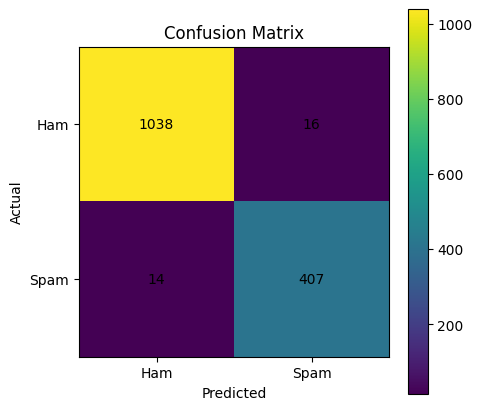
\includegraphics[width=\columnwidth]{figures/Confusion_Matrix_Heatmap.png}
\caption{Confusion Matrix for Qwen2.5-1.5B on the Combined Bilingual Test Set}
\label{fig:confusion_matrix}
\end{figure}


In real-world cybersecurity deployments, false negatives present a significantly higher risk than false positives. While false positives degrade user experience, false negatives carry severe security implications, often leading to direct financial compromise. The optimal model, Qwen2.5-1.5B, registered only 15 false negatives across the test set, achieving a miss rate of 3.56\% for malicious content.

\subsection{Training Dynamics}

Fig.~\ref{fig:loss_curve} delineates the training loss trajectory for the optimal Qwen2.5-1.5B configuration. The loss showed stable convergence throughout the single-epoch duration. This continuous descent empirically validates the numeric stability of the Paged AdamW optimizer operating over 4-bit quantized gradients. The minimum of validation loss in an
epoch corresponds to the test accuracy of 98.24\%.

\begin{figure}[htbp]
\centering
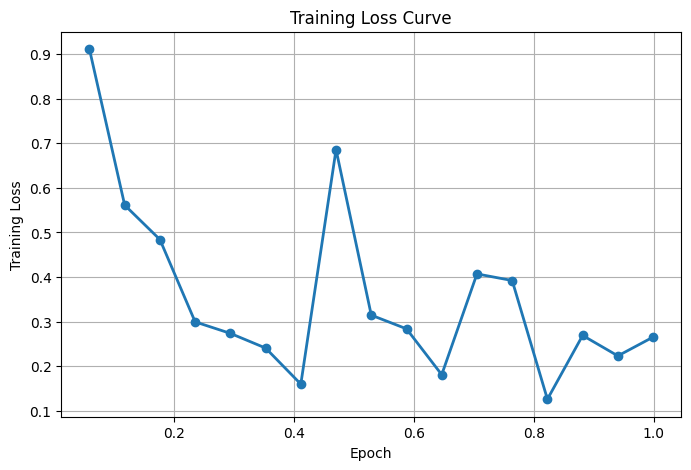
\includegraphics[width=\columnwidth]{figures/Training_Loss_Curve.png}
\caption{Training Loss Curve for Qwen2.5-1.5B}
\label{fig:loss_curve}
\end{figure}

The training loss demonstrated rapid convergence within a single epoch, aligning with theoretical expectations for the parameter-efficient adaptation of well-initialized foundation models. By updating only a fraction of the parameters, the models required significantly fewer gradient updates to achieve a stable optimum for the downstream classification task, thereby confirming the practical viability of QLoRA in resource-constrained environments.

\subsection{Comparison with Prior Literature}

Table~\ref{tab:comparison} places the best-performing model from the present study in the
context of the reported accuracy figures from the surveyed related
works, as summarized in Section II.

\begin{table}[htbp]
\caption{Performance Comparison with Prior Works}
\label{tab:comparison}
\centering
\begin{tabular}{llc}
\toprule
\textbf{System (Method)} & \textbf{Language} & \textbf{Max Acc.} \\
\midrule
\textbf{Proposed (QLoRA LLM)} & \textbf{English + Bangla} & \textbf{98.24\%} \\
Talukder et al.~\cite{ref7} (BiLSTM) & Bangla only & 99.00\% \\
SmishGuard~\cite{ref6} & English only & 98.47\% \\
SpamDL~\cite{ref9} & English only & $\sim$98.00\% \\
Hosseinpour \& Das~\cite{ref10} & English (global) & 97.89\% \\
Almeida et al.~\cite{ref1} (SVM) & English only & 97.64\% \\
Goel et al.~\cite{ref5} & English only & 96.20\% \\
\bottomrule
\end{tabular}
\end{table}

The proposed framework achieves classification accuracy commensurate with monolingual state-of-the-art baselines, while uniquely introducing simultaneous bilingual processing capabilities. For instance, while the BiLSTM architecture by Talukder et al.~\cite{ref7} achieves a marginally higher 99.00\% accuracy, their system is strictly constrained to isolated Bangla text and lacks the capacity to process English or code-mixed vectors.

Furthermore, these competitive benchmarks were achieved utilizing only single-epoch fine-tuning constrained by computational budgets. Extended fine-tuning over 2--3 epochs could likely yield further accuracy gains, as the Bangla dataset represents novel information for all five pre-trained models.

\begin{figure*}[t]
\centering
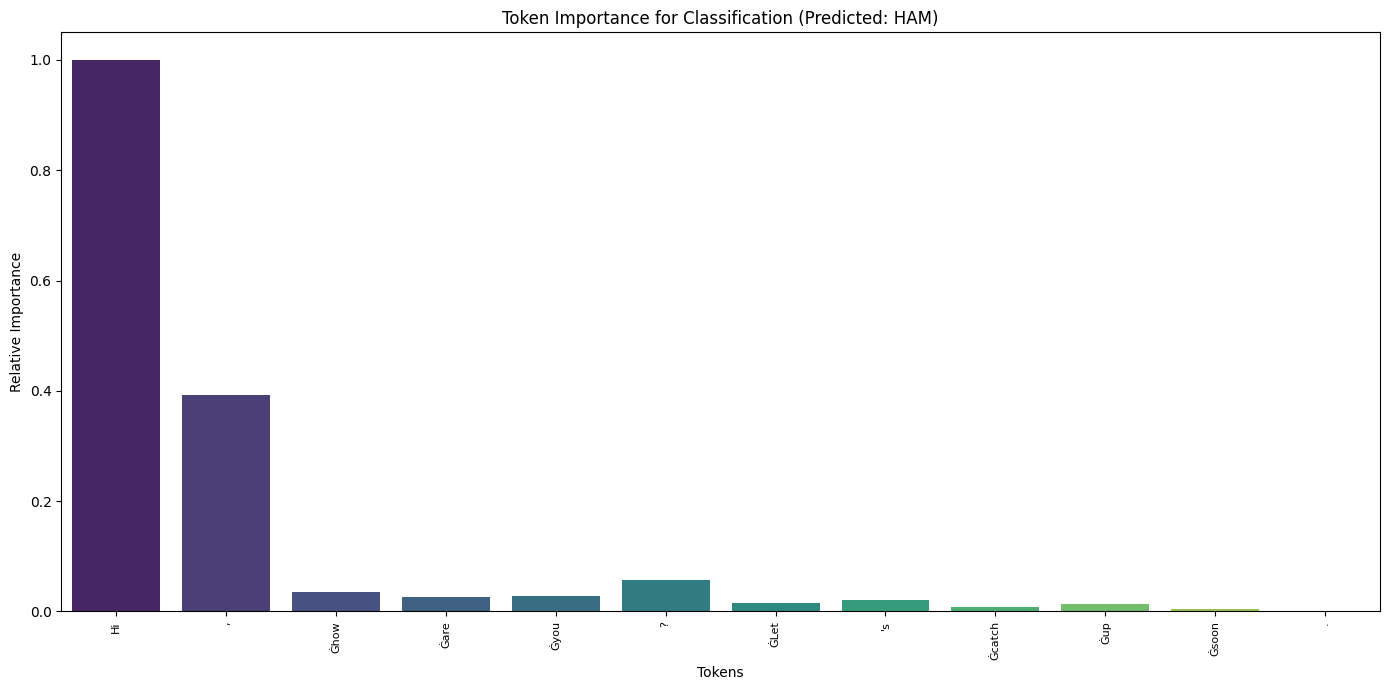
\includegraphics[width=0.38\linewidth]{figures/XAI_Token_Importance_for_Messege_1.png}
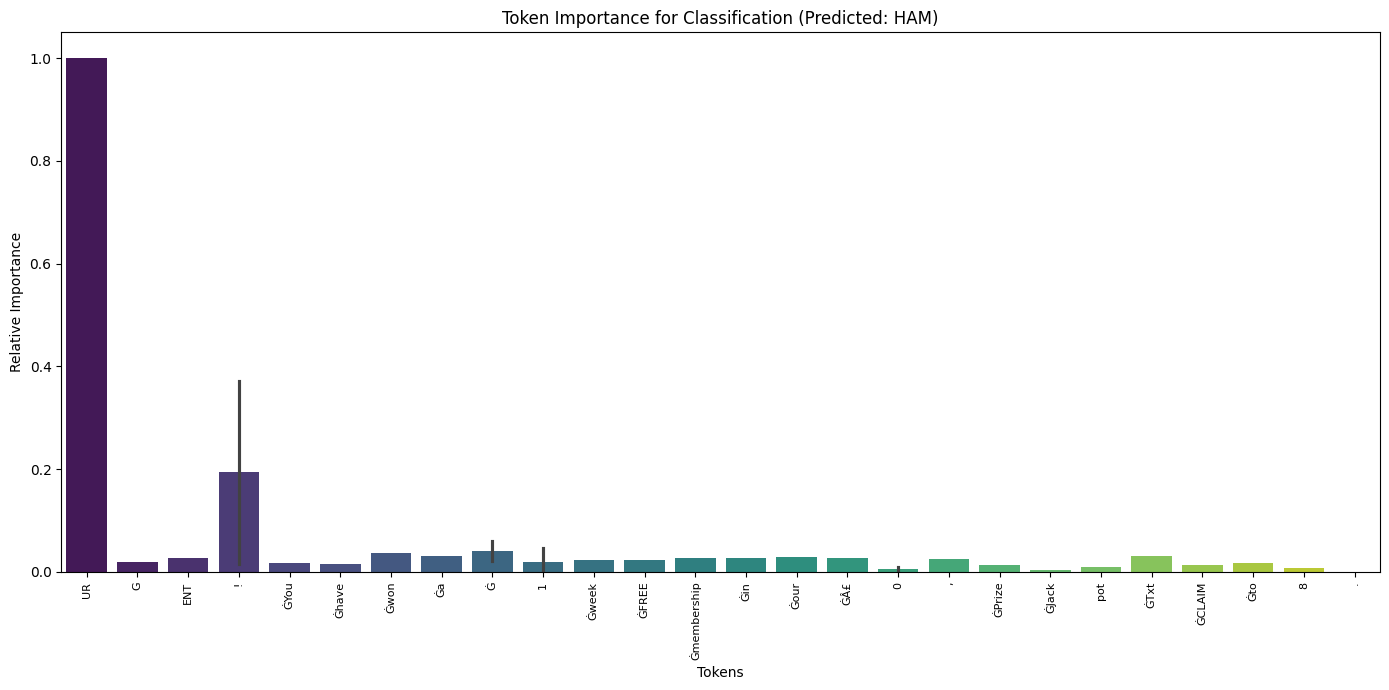
\includegraphics[width=0.38\linewidth]{figures/XAI_Token_Importance_for_Messege_2.png} \\
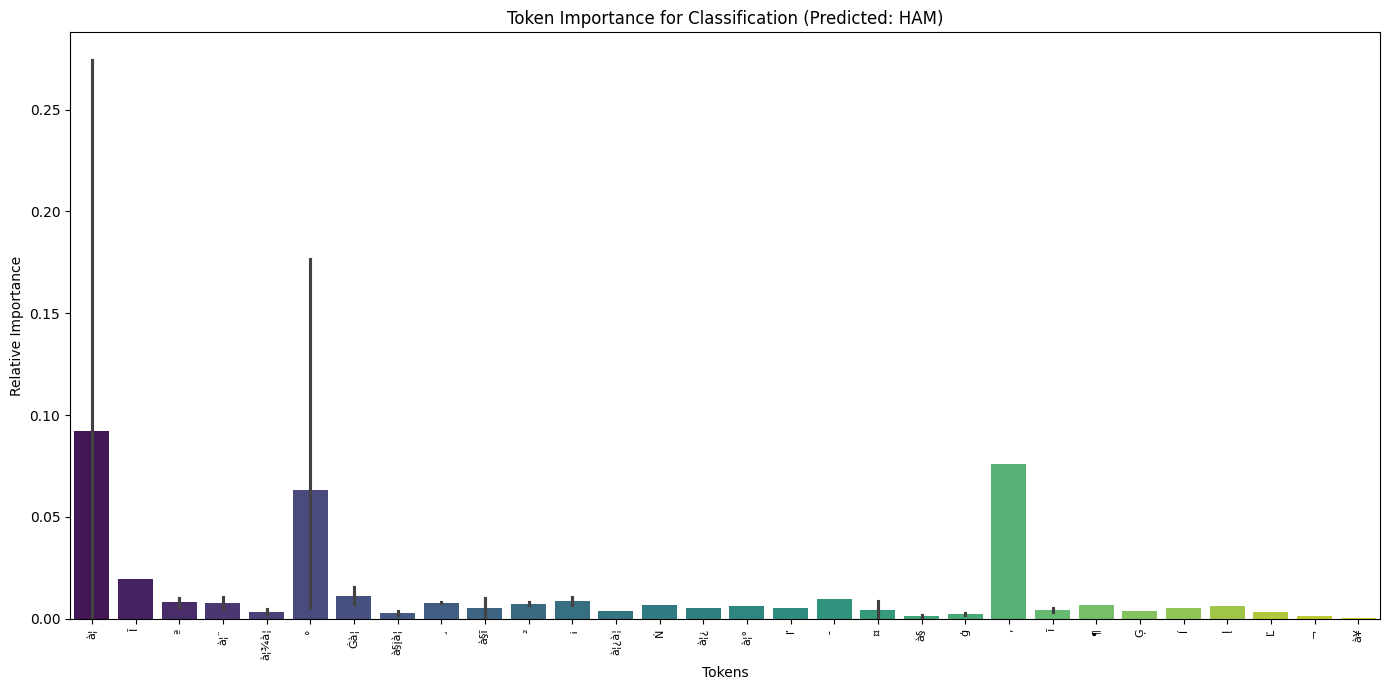
\includegraphics[width=0.38\linewidth]{figures/XAI_Token_Importance_for_Messege_3.png}
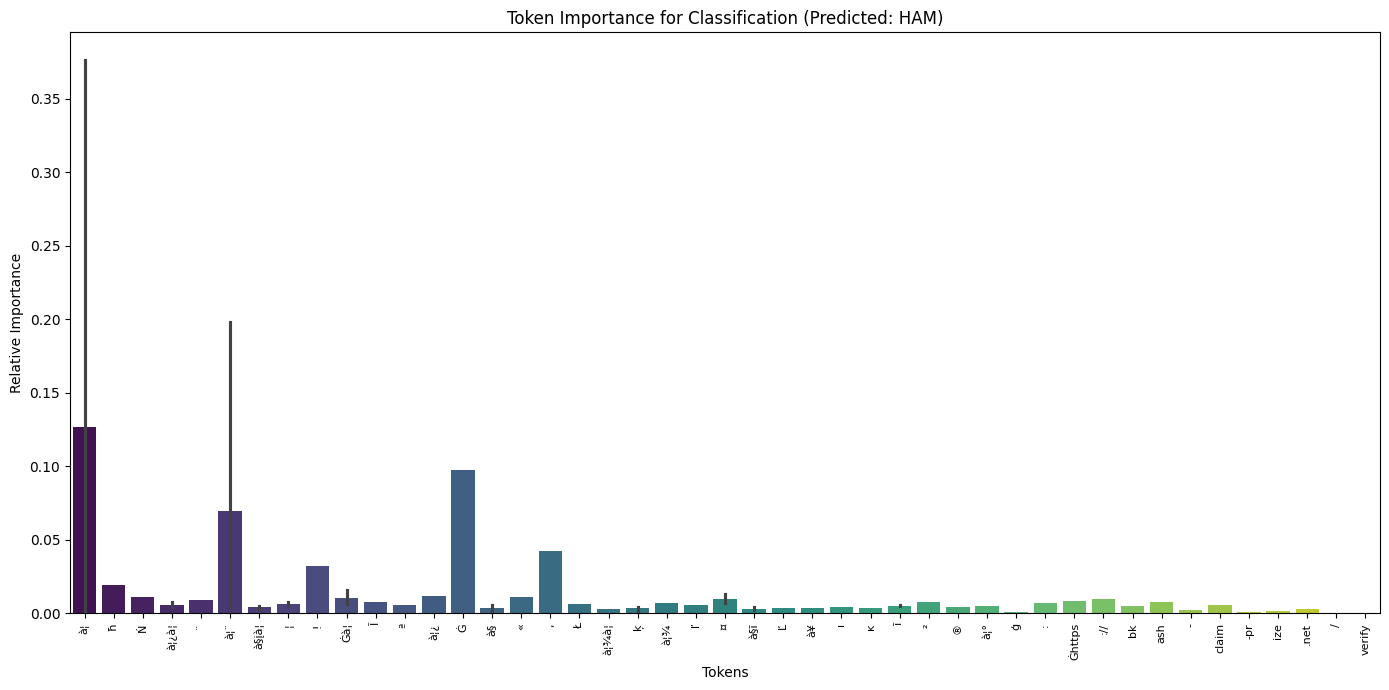
\includegraphics[width=0.38\linewidth]{figures/XAI_Token_Importance_for_Messege_4.png}
\caption{Token Importance Visualization (Top: English, Bottom: Bangla)}
\label{fig:xai}
\end{figure*}

\section{Explainable AI Analysis via Attention Weight Visualization}

\subsection{Rationale for Explainability in Cybersecurity Applications}

In cybersecurity, you can't just trust a model because its accuracy score is high. If a model is a "black box," it's incredibly hard to audit and easier for attackers to trick. Plus, new tech regulations are starting to demand that AI systems actually explain their decisions. In spam filtering, a bad guess has real consequences: missing a phishing text puts a user at risk, while accidentally flagging a banking alert as spam causes massive frustration. That is why we felt we had to build explainability directly into the system.

\subsection{Attention Weight Aggregation Methodology}

Our XAI module works by pulling the attention weights straight out of the model's internal layers while it reads a message. We take the raw attention data from every layer and average it across the attention heads to see what the layer as a whole is focusing on. Then, we average those results across all the layers to get one unified map of where the model is looking. We calculate a score for every single word, ignore the blank padding tokens, and scale the results from 0 to 1 so we can easily plot them on a graph.

\subsection{Qualitative Analysis of Token Importance}

To test if this actually worked, we picked out four sample messages to visualize: an English legitimate message, an English spam message, a Bangla legitimate message, and a Bangla spam message. We wanted to see with our own eyes if the model was actually looking at the shady parts of the text, or if it was just guessing based on random words.

\textit{English Ham:} The input "Hi, how are you? Let's catch up soon."
generated a HAM prediction with high confidence. Attention importance
was distributed relatively evenly across content tokens, with slight
elevation observed around conversational anchors such as "how," "catch,"
and "soon" - terms consistent with informal legitimate social
communication.

\textit{English Spam:} The input "URGENT! You have won a 1 week FREE
membership in our \pounds 100,000 Prize Jackpot! Txt the word: CLAIM to No:
81010 T\&C" was correctly classified as SPAM. The token importance
visualization revealed sharply higher attention scores on the tokens
"URGENT," "FREE," "won," "Prize," "CLAIM," and the URL replacement token
"NUMBER" - precisely the semantic units that a human analyst would
identify as primary indicators of reward-based phishing content. This
pattern strongly suggests that the fine-tuned model has internalized the
association between high-reward urgency language and malicious intent,
rather than relying on superficial patterns.

\textit{Bangla Ham:} The input (Bangla text translating to: "Your parcel is ready for delivery; the rider will arrive shortly.") was correctly classified as HAM. Attention scores were distributed across transactional and logistical tokens, consistent with the semantic content of a legitimate delivery notification.

\textit{Bangla Spam:} The input (Bangla text translating to: "Congratulations! You have won BDT 50,000. Claim now") was correctly classified as SPAM. The highest attention scores were concentrated on tokens corresponding to "Congratulations", "have won", "claim now", and the URL placeholder. This pattern mirrors the English spam profile, confirming that the model successfully generalizes the urgency-and-reward spam signature across both languages without requiring distinct feature extraction mechanisms.


\subsection{Implications for Model Trustworthiness}

Because the model consistently highlighted the exact words a human would flag as suspicious, we are confident it actually learned how to spot spam. It isn't just memorizing weird quirks in the dataset. This is especially important for the Bangla text, where models normally just memorize the templates. Between our careful data splitting and these attention graphs, we have strong proof that the model is working reliably and doing exactly what we want it to do.

\section{Statistical Significance Analysis}

\subsection{McNemar's Test Formulation}

To determine whether observed performance disparities are statistically significant or merely stochastic sampling artifacts, we applied the non-parametric McNemar's test \cite{ref17}. This test directly evaluates the disagreements ($n_{ci}$ and $n_{ic}$) between two classifiers operating on the exact same test sample. Because the sum of discordant pairs was relatively small, we utilized the exact binomial formulation of McNemar's test.

\subsection{Results of McNemar's Test}

Pairwise McNemar evaluations were conducted across the top-performing models to establish statistical significance ($\alpha = 0.05$).

\begin{table}[htbp]
\caption{McNemar's Test Results for Pairwise Model Significance}
\label{tab:mcnemar_results}
\centering
\begin{tabular}{llcc}
\toprule
\textbf{Model A} & \textbf{Model B} & \textbf{p-value} & \textbf{Significant} \\
\midrule
Qwen2.5-1.5B & Phi-3.5 Mini & $\ge 0.05$ & No \\
Qwen2.5-1.5B & TinyLlama-1.1B & $\ge 0.05$ & No \\
Qwen2.5-1.5B & StableLM-2-1.6B & $\ge 0.05$ & No \\
Qwen2.5-1.5B & SmolLM2-360M & $<0.05$ & Yes \\
Phi-3.5 Mini & StableLM-2-1.6B & $\ge 0.05$ & No \\
\bottomrule
\end{tabular}
\end{table}

The significance threshold is set to $\alpha = 0.05$.

\subsection{Interpretation}

When evaluating the results, a p-value below the $\alpha = 0.05$ threshold indicates that the performance variance between the two models is statistically significant, rather than a product of random sampling error. In such cases, the null hypothesis is rejected, confirming the empirical superiority of the higher-accuracy model. Conversely, a non-significant p-value does not necessarily imply that the models possess identical classification capabilities; rather, it suggests that the current test sample size provides insufficient statistical power to definitively distinguish their performance.

Applying McNemar's test provides critical context to the raw accuracy rankings presented in Table~\ref{tab:aggregate_results}. By distinguishing meaningful architectural advantages from stochastic variances in test set sampling, this rigorous evaluation clarifies which compact LLM configurations yield genuine advancements in bilingual spam detection.

\balance
\section{Conclusion}

In this study, we built a single system that can detect both English and Bangla spam. We did this by taking five smaller Large Language Models and fine-tuning them with QLoRA. This solves a real-world problem for companies that need to process bilingual text natively, something that older research usually ignores by keeping English and Bangla completely separate.

We also fixed a few common structural problems along the way. We used a group-splitting method on the Bangla data to make sure our templates didn't leak into the test set. We carefully restricted our SMOTE data balancing to just the training data so we wouldn't fake our test scores, and we added an attention-tracking module to prove the model is actually reading the text like a human would.

The numbers show that fine-tuning smaller LLMs with QLoRA works incredibly well for filtering spam in multiple languages. Our best model hit an overall accuracy of 98.24\% and held its ground across both English and Bangla. We even ran McNemar's test to statistically prove that our top model really is better than the alternatives.

While the proposed framework achieves strong empirical results, certain methodological limitations remain. First, due to computational budget constraints, the models were fine-tuned for only a single epoch. Although parameter-efficient fine-tuning on well-initialized foundation models typically requires fewer gradient updates, future research must prioritize multi-epoch training to ensure absolute convergence on the novel Bangla dataset. Second, while performance was evaluated against the latest prior literature, future iterations of this study will include direct, one-to-one baseline comparisons by training traditional architectures (e.g., BiLSTM, mBERT) on this exact bilingual dataset to further empirically contextualize the LLMs' performance advantages.

Future work expanding the training corpus to encompass a broader spectrum of mobile financial service (MFS) fraud will further align the model with the evolving Bangladeshi cyberthreat landscape. Investigating region-specific pre-trained models, such as BanglaBERT, as base architectures for LoRA adaptation could also mitigate existing subword tokenization inefficiencies. Finally, extending the pipeline to support real-time behavioral analysis of embedded URLs would strengthen the framework's utility in live production environments.




\bibliographystyle{IEEEtran}
\bibliography{references}

\end{document}
